\chapter{Números/Relações (2º Bimestre)}

\section{Equações de 2º grau}

A equação quadrática pode ser escrita como
$$a x^2 + b x + c = 0$$
onde $a, b, c$ são constantes reais,
$a \neq 0$ e $x$ é o número desconhecido.
Desejamos determinar o valor de $x$ que satisfaça a igualdade
que é chamada de solução da equação.

Por exemplo,
para $a=3, b=3, c=-18$ temos que
$1$ não é solução pois
$3 \times 1^2 + 3 \times 1 - 18 = -12 \neq 0$
mas $2$ é solução pois $3 \times 2^2 + 3 \times 2 - 18 = 12 + 6 - 18 = 0$.
Também podemos verificar que $-3$ é outra solução.

Temos que
$$a x^2 + b x + c =
a \left( x^2 + \frac{b}{a} x + \frac{c}{a} \right) =
a \left( x^2 + 2 \frac{b}{2a} x + \left(\frac{b}{2a}\right)^2
- \left(\frac{b}{2a}\right)^2 + \frac{4ac}{4a^2} \right)
$$
Se escrevermos $\Delta = b^2 - 4ac$ obtemos
$$a x^2 + b x + c =
a \left( \left(x + \frac{b}{2a}\right)^2 - \frac{\Delta}{4a^2} \right)$$
Para $\Delta < 0$ temos que
$\left( \left(x + \frac{b}{2a}\right)^2 - \frac{\Delta}{4a^2} \right) > 0$
para qualquer número real $x$ e a equação quadrática não possui solução.
Se $\Delta = 0$, a equação torna-se
$$\left(x + \frac{b}{2a}\right)^2 = 0$$
e a equação possui uma única solução $x = -\frac{b}{2a}$.
Finalmente, se $\Delta > 0$  podemos escrever
$$\left(x + \frac{b}{2a}\right)^2 = \left(\frac{\sqrt{\Delta}}{2a}\right)^2$$
tal que $x + \frac{b}{2a} = \frac{\sqrt{\Delta}}{2a}$ ou
$x + \frac{b}{2a} = -\frac{\sqrt{\Delta}}{2a}$.
Finalmente, obtemos duas soluções
$$x = \frac{-b \pm \sqrt{b^2 - 4ac}}{2a}$$

\subsection*{Exercício 1}

Resolva as equações a seguir:

\begin{enumerate}
\item $y^2 - 5y - 14 = 0$
\item $u^2 - \frac{9}{2}u - 9 = 0$
\item $3t^2 - \frac{222}{5}t - 9 = 0$
\item $v^2 + {(\sqrt3 - 8)}v - 8\sqrt3 = 0$
\item $25z^2  - 10\sqrt7 z  + 7 = 0$
\item $-2r^2 + 8r - 26 = 0$
\end{enumerate}

\subsection*{Exercício 2}

João possui uma casa quadrada que possui dois quartos com uma área total de $x^2$m².
O primeiro quarto é um retângulo de dimensão $3 \times x$
e o segundo possui área igual a $59$m².
Qual é a área total dessa cada?

\section{Funções e variação}

Para definirmos uma função $f$,
associamos a cada número real $x$ um outro número real $f(x)$.
$f(x)$ é chamado image de $x$ em $f$.
Por exemplo,
$f(0) = 1$,
$f(x) = \sqrt{x}$ se $x > 0$
e $f(x) = -\frac{1}{x}$ se $x < 0$.

Se para qualquer números $x$ e $y$ reais tal que $x < y$
temos $f(x) \leq f(y)$ dizemos que a função $f$ é crescente.
Se tivermos a condição $f(x) < f(y)$ para todo $x < y$
dizemos que $f$ é estritamente crescente.
De forma semelhantes,
definimos função decrescente e função estritamente decrescente
se tivermos satisfeita, respectivamente, as condições
$f(x) \geq f(y)$ 
e $f(x) > f(y)$
para todo $x < y$.
Por exemplo,
a função $f$ definida por $f(x) = x^3$ is estritamente crescente e
a função $g$ definida por $g(x) = -x$ é estritamente decrescente.

Funções também pode ser definidas para um subconjunto dos números reais.
Por exemplo,
$f(x) = \sqrt{x}$ é definida para todos os números reais não negativos.
De forma semelhante,
funções crescentes e decrescentes também podem ser definida para subconjuntos dos reais.
Por exemplo,
a função $f(x) = \left| x \right|$
é crescente para os números negativos
e é crescente para os números positivos.

Quando $x$ aproxima-se de um número real $a$,
o valor $f(x)$ pode
\begin{enumerate}
  \item ficar tão próximo de um número real $L$ quanto se desejar e dizemos que
    $f$ possui um limite $L$ no ponto $a$,
  \item ficar maior que qualquer número real e dizemos que $f$ possui limite
    infinito ou $\infty$ no ponto $a$,
  \item ficar menor que qualquer número real negativo e dizemos que $f$ possui
    menos limite  ou $-\infty$ no ponto $a$.
\end{enumerate}
Podemos fazer a distinção entre $x$ aproximar-se de $a$
pelos valores a esquerda ($f$ possui limite no ponto $a^-$)
ou pelos valores a direita ($f$ possui limite no ponto $a^+$).
De forma similar, podemos definir um limite de $d$ em $\pm\infty$,
isso é, quando $x$ assume valores, em valor absoluto, grandes.

Por exemplo,
se definirmos para todo $x \neq 0$ a função $f(x) = \frac{1}{x}$
então o limite de $d$ nos pontos $-\infty, 0^-, 0^+, +\infty$ é,
respectivamente, $0, -\infty, +\infty, 0$.

\subsection*{Exercício 3}

Determine a imagem de $-1$, $0$ e $1$ para as funções a seguir:

\begin{enumerate}
  \item $f(x) = \pi$
  \item $g(x) = 8$ se $x < 0$, $g(x) = -7$ se $x > 0$ e $g(0) = 5$.
  \item $h(x) = -2x + 3$
  \item $i(x) = 2x^2 - 5x + 9$
  \item $j(x) = \sqrt{x+8}$ se $x > 0$ e $j(x) = -6x$ se $x \leq 0$.
\end{enumerate}

\subsection*{Exercício 4}

Indique o maior subconjunto dos números reais
para o qual as funções a seguir estão definidas.
Descreva a variação da função,
isso é, dizer em qual intervalo a função cresce ou decresce.

\begin{enumerate}
  \item $f(x) = -4x + 2$
  \item $g(x) = 6 - \frac{1}{x^2}$
  \item $h(x) = \sqrt{x+6}$
\end{enumerate}

Qual o limite das funções $f$ e $g$ em $+\infty$ e $-\infty$?
Qual o limite de $h$ em ${-6}^+$ e $-\infty$?
E qual o limite de $g$ em $0$?

\subsection*{Exercício 5 (difícil)}

Definimos a função $f$ por $f(x) = 0$ se $x$ é um racional e
$f(x) = 1$ caso contrário. A função $E$ é definida como:
$E(x)$ é o único inteiro tal que
$E(x) \leq x < E(x) + 1$.

\begin{enumerate}
\item Calcule $f(0)$ e $f(\sqrt{2})$.
\item Calcule $E(2)$, $E(-4,5)$ e $E(1,5)$.
\item Considere um número real $a$ e defina a função $g$ dad por
  $g(n) = \frac{E(\sqrt{2}^n a)}{\sqrt{2}^n}$ para todo inteiro $n$.
  Determine $f(g(n))$ para quando o valor de $n$ é par ou ímpar.
\item Qual é o limite de $g(n)$ quando $n$ se aproxima de $+\infty$ por meio de
  números inteiros pares? E por números inteiros ímpares?
\item É possível que $f$ tenha um limite no ponto $a$?
\item Considere um intervalo real não vazio $(A, B)$ e
  defina $a_1 = \frac{3A+B}{4}$ e $a_2 = \frac{A+3B}{4}$.
  Ordene $A,B,a_1,a_2$.
\item Mostre que existe $x$ próximo o suficiente de $a_1$ e
  $y$ próximo o suficiente de $a_2$ tal que
  $x < y$ e $f(x) < f(y)$.
  Prove essa afirmação com $f(x) > f(y)$.
\item O que pode ser dito sobre a variação de $f$ no intervalo $(A,B)$?
\end{enumerate}

\section{Tabelas e gráficos}

Considere a função $f$ e alguns números reais
$x_1 = -\infty, x_2, \ldots x_n = +\infty$
tal que $f$ é definido e monótono (crescente ou decrescente) para cada intervalo
definido por $(x_i, x_{i+1})$ e que possui limite no ponto $x_i$.
Podemos criar uma tabela de variações com duas linhas.
A primeira linha contem os pontos $x_i$ e a segunda linha o limite de $f$
nesses pontos. Na segunda linha, utilizamos setas para indicar se a função é
crescente ou decrescente. Como um exemplo, a função
$f(x) = {|x|} + \pi$
pode ser descrita pela seguinte tabela:

\begin{center}
  \begin{tabular}{|c c c c c|}
    \hline
    $-\infty$ & & $0$   &  & $+\infty$ \\
    \hline
    $+\infty$ & $\searrow$ & $\pi$ & $\nearrow$ & $+\infty$ \\
    \hline
  \end{tabular}
\end{center}

Podemos desenhar o gráfico de uma função no plano cartesiano como um conjunto de
todos os pontos de coordenadas $(x, f(x))$ para os quais a função está definida.
Por exemplo, a função $f(x) = x$ e $g(x) = x^2$ são desenhadas como uma linha
reta e uma parábola.

\begin{center}
  \begin{tikzpicture}[domain=-2:2]
    \draw[->] (-3,0) -- (3,0) node[right] {$x$}; 
    \draw[->] (0,-2) -- (0,5) node[above] {$y$};
    \draw[color=blue] plot (\x,\x*\x) node[left] {$g$};
    \draw[color=red] plot (\x,\x) node[left] {$f$};
    \foreach \x in {-2,-1,1,2}
      \draw (\x,-.1) --(\x,.1) node[above] {$\x$};
    \foreach \y in {-2,-1,1,2,3,4}
      \draw (-.1,\y) --(.1,\y) node[left] {$\y$};
  \end{tikzpicture}
\end{center}

Seja $a$, $b$ constantes reais e $h$ a função linear $h(x) = ax + b$.
Se $a = 0$, então $f$ é constante no valor $b$ e o gráfico é uma linha
horizontal com todos os pontos tendo ordenada igual $b$.
Se $x_1 < x_2$ então $ax_1 < ax_2$ se $a > 0$ e $ax_2 > ax_1$ se $a < 0$.
Deduzimos que $h$ é (estritamente) crescente ou decrescente de acordo com o
valor de $a$ ser positivo ou negativo. O gráfico de $h$ é obtido da linha reta
representando $f$ depois de aplicar um escalonamento de fator $a$ e transladar o
gráfico em $b$ para cima. De forma similar,
se $i(x) = ax^2 + bx + c$, podemos ver que
%%
$$i(x) = a x^2 + b x + c =
a \left( \left(x + \frac{b}{2a}\right)^2 - \frac{\Delta}{4a^2} \right)$$

onde $\Delta = b^2 - 4ac$. Isso significa que o gráfico de $i$ é obtido ao
transladar a parábola representando $g$ acima em $\frac{b}{2a}$ para a direita e
$\frac{\Delta}{4a^2}$ para baixo e finalmente aplicar o escalonamento de fator $a$

\subsection*{Exercício 6}

Identifique os gráficos de
$y = 10$,
$y=-2x+15$,
$y=-2x+5$,
$y=2x+10$,
$y=3x+10$ e
$y=\frac{x^2}{10} + 10$
na figura a seguir:

\begin{center}
  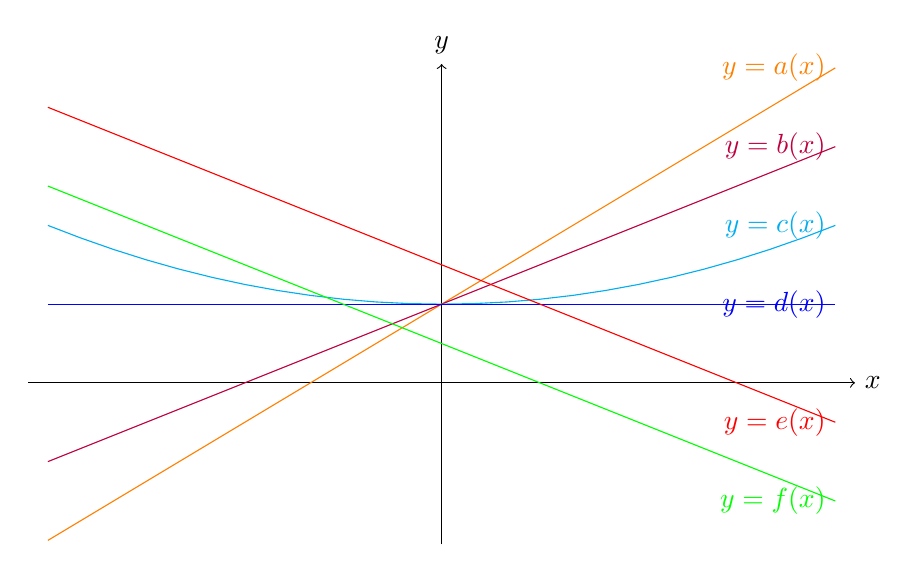
\begin{tikzpicture}[domain=-10:10, xscale=.5, yscale=0.1]
    \draw[->] (-10.5,0) -- (10.5,0) node[right] {$x$}; 
    \draw[->] (0,-20.5) -- (0,40.5) node[above] {$y$};
    \draw[color=orange] plot (\x,{3*\x + 10}) node[left] {$y=a(x)$};
    \draw[color=purple] plot (\x,{2*\x + 10}) node[left] {$y=b(x)$};
    \draw[color=cyan] plot (\x,{\x*\x/10 + 10}) node[left] {$y=c(x)$};
    \draw[color=blue]    plot (\x,10)       node[left] {$y=d(x)$}; 
    \draw[color=red]   plot (\x,{-2*\x + 15})    node[left] {$y=e(x)$}; 
    \draw[color=green] plot (\x,{-2*\x + 5}) node[left] {$y=f(x)$};
  \end{tikzpicture}
\end{center}

\subsection*{Exercício 7}

Trace o gráfico das funções quadráticas a seguir.
Indique os pontos de máximo, mínimo e os zeros.
O que é possível dizer sobre a forma das parábolas?

\begin{enumerate}
\item $f(x) = \frac{x^2}{4} - \frac{x}{2}$
\item $g(x) = -\frac{x^2}{4} - \frac{x}{2} - \frac{1}{2}$
\end{enumerate}

\section{Solução dos Exercícios}

\subsection*{Exercício 1}

\begin{enumerate}
\item $y = 7$ ou $y=-2$
\item $u = 6$ ou $u = -\frac{3}{2}$
\item $t = 15$ ou $t = -\frac{1}{5}$
\item $v = 8$ ou $v = -\sqrt{3}$
\item $z = \frac{\sqrt{7}}{5}$
\item A equação não possui nenhuma solução real.
\end{enumerate}

\subsection*{Exercício 2}

$3x + 59 = x^2$ é equivalente a $x^2 - 3x - 59 = 0$.
Então $\Delta = 245 > 0$ e
$$x=\frac{3 \pm 7 \sqrt5}{2}$$
Obtemos que $x \approx -6.33$m ou $x\approx9.33$m.
Como $x > 0$ ficamos apenas com a solução positiva.
A área total é
$$
x^2 = \frac{21 \sqrt5+127}{2} \approx 87 \text{m²}
$$

\subsection*{Exercício 3}

\begin{enumerate}
  \item $f(-1) = f(0) = f(1) = \pi$
  \item $g(-1) = 8$, $g(1) = -7$ e $g(0) = 5$
  \item $h(-1) = 5$, $h(0) = 3$ e $h(1) = 1$.
  \item $i(-1) = 16$, $i(0) = 9$ e $i(1) = 6$.
  \item $j(1) = \sqrt{9} = 3$, $j(x) = 0$ e $j(-1) = 6$.
\end{enumerate}

\subsection*{Exercício 4}

\begin{enumerate}
  \item $f$ é definido para todo o conjunto dos reais.
    Se $x < y$ então $-4 x > -4 y$ e portanto $f(x) > f(y)$.
    $f(x)$ é estritamente crescente.
  \item $g(x)$ é definida para todo $x \neq 0$.
    Se $0 < x < y$ então $0 < x^2 < y^2$,
    $frac{1}{x^2} > \frac{1}{y^2}$,
    $-\frac{1}{x^2} < -\frac{1}{y^2}$
    e finalmente $g(x) < g(y)$.
    Então $g$ é estritamente crescente no conjunto do números reais positivos.
    De forma similar, $g$ é estritamente decrescente no conjunto dos números
    reais negativos
  \item $h(x)$ é definido se $x+6 \geq 0$,
    isso é,
    para todos os reais tal que $x \geq -6$.
    Se $-6 \leq x < y$ então $0 \leq x + 6 < y + 6$
    e portanto $h(x) < h(y)$.
    Logo, $h$ é estritamente crescente.
\end{enumerate}

Se $x$, em valores absolutos, é grande,
então $-4x$ é um valor grande com sinal oposto.
Assim sendo, o limite de $f$ em $+\infty, -\infty$ é, respectivamente, $-\infty, +\infty$.

Se $x$, em valores absolutos, é grande,
então $x^2$ também é grande e
e $-\frac{1}{x^2}$ é um valor pequeno negativo..
Assim sendo, o limite de $g$ em $+\infty, -\infty$ é $6^{-}$.

O limite de $h$ em ${-6}^+, +\infty$ é $h(6) = 0, +\infty$.
Se $x$ assume valores próximos de $0$ então $x^2$ é valores positivos próximos
de $0$ e assim $-\frac{1}{x^2}$ assume valores grandes negativos.
Então o limite de $g$ em $0$ é $-\infty$.

\subsection*{Exercício 5 (difícil)}

Definimos a função $f$ por $f(x) = 0$ se $x$ é racional
e $f(x) = 1$ caso contrário.
A função $E$ é definida como indicado a seguir:
$E(x)$ é o único inteiro tal que $E(x) \leq x < E(x) + 1$.

\begin{enumerate}
\item $f(0) = 0$ (pois $0$ é um racional)
  e $f(\sqrt{2}) = 1$
  (porque $\sqrt{2}$ é irracional, ver primeiro bimestre).
\item $E(2) = 2$, $E(-4.5) = -5$ e $E(1.5) = 1$.
\item $E(\sqrt{2}^n a)$ é sempre um inteiro por definição.
  Se $n$ é par, então $\sqrt{2}^n$ também é um inteiro.
  Já $g(n)$ é um racional e $f(g(n)) = 0$.
  Se $n$ é par,
  então $g(n) = \frac{E(\sqrt{2}^n a)}{\sqrt{2}^{n+1} a} \sqrt{2}$
  e a fração é um racional.
  Como consequência $g(n)$ pode não ser um racional ou será $\sqrt{2}$.
  Finalmente, $f(g(n)) = 1$.
\item Temos a desigualdade $E(\sqrt{2}^n a) \leq a < E(\sqrt{2}^n a) + 1$
  e dividindo por $\sqrt{2}^n$ obtemos
  $g(n) \leq a < g(n) + \frac{1}{\sqrt{2}^n}$ que é
  $$0 \leq a - g(n) < \frac{1}{\sqrt{2}^n}$$

  $\frac{1}{\sqrt{2}^n}$ pode ser próximo de $0$ o quanto desejarmos
  quando $n$ é grande e assim o limite de $g(n)$ no $+\infty$ é $a$
  (tanto se considerarmos os valores pares e ímpares).

\item Se $L$ é um limite, então $n$ aproxima-se de $+\infty$ por valores
  inteiros pares, então $g(n)$ aproxima-se de $a$ e portanto $f(g(n))$
  aproxima-se de $L$.
  Mas como $f(g(n))$ assume o valor constante $0$ que implica em $L = 0$.
  De maneira similar, se considerarmos números inteiros ímpares iremos deduzir
  que $L = 1$.
  Isso é uma contradição, então $f$ não pode ter limite no ponto $a$.
\item Temos $A<B$ e portanto
  $A = \frac{3A+A}{4} < \frac{3A+B}{4} = a_1 < a_2 < 
  \frac{A+3B}{4} < \frac{B+3B}{4} = B$.

\item Considerando $x = \frac{E(\sqrt{2}^{2n} a_1)}{\sqrt{2}^{2n}}$ e
  $y = \frac{E(\sqrt{2}^{2n+1} a_2)}{\sqrt{2}^{2n+1}}$
  para valores grandes de $n$.
  Então $x$ é próximo o suficiente de $a_1$ e
  $y$ é próximo o suficiente de $a_2$
  de modo que temos $x < y$.
  Além disso, $x$ é racional e $y$ é irracional
  e assim $f(x) = 0 < 1 = f(y)$.
  Obtemos valores tal que $f(x) > f(y)$ ao trocar os parâmetros inteiros
  ímpares por pares e vice-versa.
\item Pela questão anterior, $f$ não é nem crescente nem decrescente no
  intervalo $(A, B)$.
\end{enumerate}

\subsection*{Exercício 6}

O gráfico de $c(x)=\frac{x^2}{10} + 10$ não é uma reta.
$d(x) = 10$ é constante e corresponde a reta paralela ao eixo $X$.
As retas de $a(x) = 3 x + 10$ e $b(x) = 2 x + 10$ encontram-se no eixo $y$ no
ponto $y = 10$ sendo que a primeira cresce mais rápido que a segunda
porque $3 > 2$. As retas paralelas são as de $e(x) = -2x + 15$ e
$f(x) = -2x + 5$ e as funções são decrescentes (possuem o mesmo $a = -2 < 0$).
A primeira reta está acima porque $15 > 5$.

\subsection*{Exercício 7}

\begin{enumerate}
\item $f(x) = \frac{1}{4} \left(x-1\right)^2 - \frac{1}{4}$. Mínimo
$-\frac{1}{4}$ em $x = 1$. A parábola possui abertura para cima
e encontra o eixo $X$ em $x = 0$ e $x = 2$.
\item $g(x) = -\frac{1}{4} \left(x+1\right)^2 - \frac{1}{4}$. Máximo
$-\frac{1}{4}$ em $x = -1$. A parábola possui abertura para baixo
e não encontra o eixo $X$.
\end{enumerate}

\begin{center}
 \begin{tikzpicture}[domain=-5:5]
   \draw (0,0) node[above] {$0$};
   \draw[->] (-5,0) --(5,0) node[above] {$x$};
   \draw[->] (0,-5) --(0,5) node[right] {$y$};
   \draw[color=orange] plot[domain=-3:5] (\x,.25 * \x * \x - .5 * \x) node[left] {$y=f(x)$};
   \draw[color=blue] plot[domain=-5:3] (\x,-.25 * \x * \x - .5 * \x - .5) node[left] {$y=g(x)$};
    \foreach \x in {-4,-3,-2,-1,1,2,3,4}
      \draw (\x,-.1) --(\x,.1) node[above] {$\x$};

    \foreach \y in {-4,-3,-2,-1,1,2,3,4}
      \draw (-.1,\y) --(.1,\y) node[right] {$\y$};

   \draw[style=dashed,color=red] (-1,0) --(-1,-.25) -- (0, -.25) node[below] {$-\frac{1}{4}$} -- (1,-.25) -- (1,0);

 \end{tikzpicture}
\end{center}
